\documentclass{mywork}

	\addtolength{\headheight}{\baselineskip}
	\lhead{Proseminar – Bézier- und B-Spline-Kurven\\ 31. Mai 2013}
%	\chead{Der Algorithmus von de Casteljau}
	\rhead{\theauthor \\}
	\cfoot{\thepage}


\begin{document}

\section*{Der Algorithmus von de Casteljau}


\subsection*{Einführung}

Der Algorithmus von de Casteljau erlaubt eine rekursive Berechnung der Kurvenpunkte auf einer Bézier-Kurve.
Im Folgenden seien stets $c_0, c_1, \dotsc, c_n$ die Kontrollpunkte der Bézier-Kurve $p(t) = \sum_{j=0}^n c_j b_j^n(t)$.

\subsection*{Visualisierung}

\begin{figure*}[h]
	\centering
	%\caption{Darstellung der Konstruktion eines Kurvenpunktes für $t = 0.5$}
	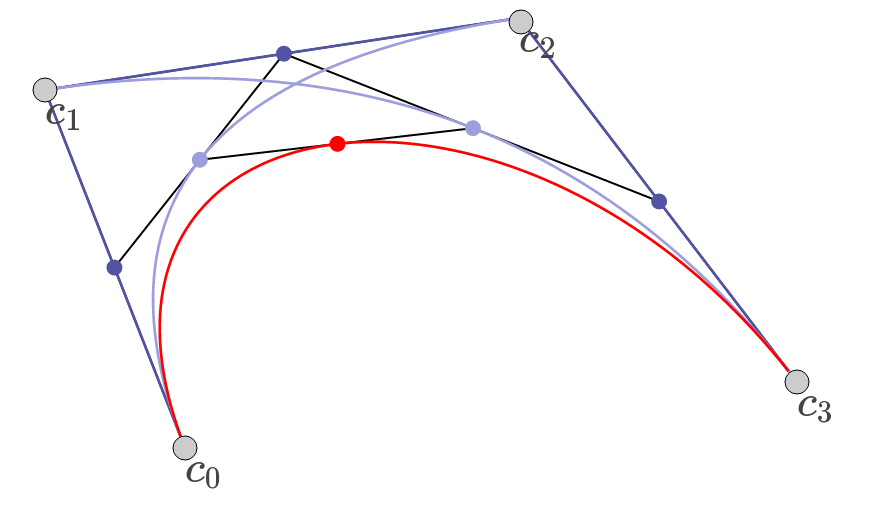
\includegraphics[scale=0.3]{casteljau.png}
\end{figure*}

\subsection*{Definitionen}

Wir bezeichnen die Bézier-Kurven, welche aus den Kontrollpunkten $c_k, c_{k+1}, \dotsc, c_{k+m}$ ($0\le k \le n, \; 0 \le m \le n - k$) gebildet werden als $p_k^m(t)$:
\[
	p_k^m(t) := \sum_{j=0}^m c_{k+j} b_j^m(t)
\]
Insbesondere entsprechen der Bézier-Kurve zu $c_0, \dotsc, c_n$ gerade $p_0^n(t)$ und den Kontrollpunkten $c_k$ gerade die $p_k^0(t)$:
\begin{align*}
	p_0^n(t) &= p(t), \\
	p_k^0(t) &= c_k.
\end{align*}

\subsection*{Rekursion und Algorithmus}

Die $p_k^m(t)$ erfüllen die Rekursion
\[
	p_k^m(t) = (1-t) \cdot p_k^{m-1}(t) + t \cdot p_{k+1}^{m-1}(t).
\]
Mit anderen Worten: man erhält den Punkt $p_k^m(t)$, indem man die Strecke $\overline{p_k^{m-1}(t)p_{k+1}^{m-1}(t)}$ im Verhältnis $t$ zu $1-t$ teilt.

\begin{proof}
	Erfolgt durch Einsetzen der Rekursion für die Bernsteinpolynome in die Definition der $p_k^m(t)$ und anschließender Umformung.
\end{proof}

\newpage

\subsection*{Anwendungen}


\begin{itemize}
	\item
		Rekursive, numerisch stabile Berechnung von Kurven-Punkten auf einer Bézier-Kurve
	\item
		Aufspalten einer Bézier-Kurve an einem beliebigen Punkt auf der Kurve in zwei einzelne Bézier-Kurven, welche zusammengesetzt genau den Verlauf der ursprünglichen beschreiben.

		Wähle dazu $(p_0^k(t))_{k=0}^n$ als Kontrollpunkte der ersten und $(p_{n-k}^k(t))_{k=0}^n$ als Kontrollpunkte der zweiten Bézier-Kurve.
	\item
		Erlaubt einfache geometrische Konstruktion von Kurven-Punkten mit Zirkel und Lineal.
\end{itemize}



\end{document}
